\section{Reproduction of results in paper}

We chose to reproduce figure 2c from the Wang et. al paper which highlights the behavior of the model and biological interpretation. For a description of our attempt to recreate figure 3c, see the appendix.

Figure 2c is a plot of cancerous crypt probability against time with varying parameters. 
\begin{figure}[h]
    \centering
    % First image
    \begin{minipage}{0.45\textwidth}
        \centering
        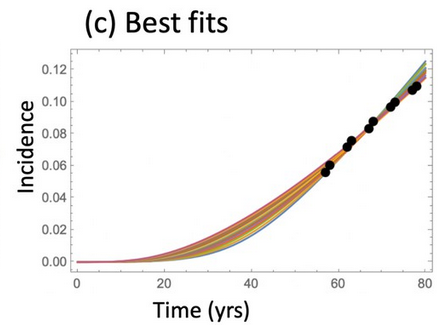
\includegraphics[width=\textwidth]{figures/Fig2c_actual.png}
    \end{minipage}
    \hfill
    % Second image
    \begin{minipage}{0.45\textwidth}
        \centering
        \includegraphics[width=\textwidth]{figures/Fig2c_Recreate.png}
    \end{minipage}
    \caption{Left, figure 2c. from Wang et. al paper. Right, recreation of figure 2c. Plot of cancerous crypt incidence curves.}
    \label{fig:side_by_side}
\end{figure}

\FloatBarrier
To obtain this probability, we use the solution of the last ODE in our system which gives the probability of having at least one crypt with all the necessary cancerous mutations at time t,

\begin{equation}
    \dot{P} = (R_{56}+R_{36}n3)(1-P), \quad P(0)=0
\end{equation}

However, small populations of type 6 crypts are not detectable. Thus epidemiological data is limited to the incidence of having a detectable number of type 6 crypts, by which time a patient is diagnosed with cancer. The paper uses a time shift to define the incidence,
\begin{equation}
    I(t) = P(t-\Delta T) * (1-\delta/\gamma_6)
\end{equation}
Where $\delta$ is the cell death rate, $\gamma_6$ is the fission rate for type 6 crypts, and  $\Delta T$ is the estimated time to detection, 4.79 years.

From this figure, we see that the ODE model is in good agreement with observed epidemiological data as we predict very similar incidence probabilities as the sample experimental incidence. The spectrum of curves is obtained by varying stem cell division rate ($r_1$), $K_A$, and $K_R$ values simultaneously. Because discrete incidence probabilities are used to fit a continuous curve, our model allows predictive estimates of the number of individuals who have at least one cancerous crypt at ages outside our discrete range. For example, the graph highlights the importance of early screening for CRC as by age forty, approximately two in every one hundred individuals will have acquired at least one cancerous crypt, even though they may not be experiencing symptoms. 
It is worth noting that while the figure description asserts that the figure only varies $r_1$, the supplied mathematica code seems to suggest division rate and carrying capacity were varied in tandem, and this procedure was necessary to produce the same diverging behavior at short and long times, and converging behavior around the incidence data. 


\begin{table}[h]
  \centering
    \begin{tabular}{l|*{5}r}
    \toprule
    \multicolumn{6}{c}{SSE Values for Best Parameter Sets} \\
    \midrule
    \diagbox{Set}{Params} & $r$ & $K_A$ & $K_R$ & $SSE$ \\
    \midrule
    $Best$ & $156$ & $562$  & $1780$ & $4.63 * 10^{-5}$ &\\ 
    $2$ & $168$ & $17$ & $1330$  & $5.22 * 10^{-5}$ &  \\ 
    $3$ & $168$ & $13$ & $1330$ & $5.22* 10^{-5}$ &  \\ 
    $4$ & $168$ & $10$ & $1330$ & $5.22 * 10^{-5}$ &  \\ 
    $5$ & $168$ & $23$ & $1330$ & $5.22 * 10^{-5}$ &  \\ 
    \bottomrule
    \end{tabular}
    \caption{5 best parameter sets from varing $r$,$K_A$, and $K_R$.}
    \label{tab:empty_table}
\end{table}

    %$6$ & $168$ & $31$ & $1330$ & $5.22 * 10^{-5}$ &  \\ 
    %$7$ & $168$ & $42$ & $1330$ & $5.22 * 10^{-5}$ &  \\ 
    %$8$ & $168$ & $56$ & $1330$ & $5.23 * 10^{-5}$ &  \\ 
    %$9$ & $168$ & $75$ & $1330$ & $5.23 * 10^{-5}$ &  \\ 
    %$10$ & $174$ & $422$ & $1000$ & $5.34 * 10^{-5}$ &  \\
    
\FloatBarrier 

Table 1 displays the sum of squared error (SSE) between a given curve and the observed data points for the five best parameter sets from our fitting procedure. Cell division rate was varied between 150 and 270 and K values were varied from 10 to 3000. From this table, we can see that for a crypt size of $10^7$, predicted stem cell division rates are fairly low, and in most cases the carrying capacity for $K_A$ APC first cells was lower than the $K_R$, the carrying capacity for KRAS first cells. 

These incidence curves and associated parameters verify the accuracy of our model, highlights it's predictive power, and may reveal the behavior of intracrypt dynamics.
